\documentclass[11pt]{article}

% ---------- Packages ----------
\usepackage[margin=1in]{geometry}
\usepackage[T1]{fontenc}
\usepackage[utf8]{inputenc}
\usepackage{lmodern}
\usepackage{setspace}
\usepackage{hyperref}
\usepackage{graphicx}
\usepackage{booktabs}
\usepackage{enumitem}
\usepackage{caption}
\usepackage{subcaption}
\usepackage{xcolor}
\usepackage{listings}
\usepackage{amsmath,amssymb}
\usepackage{cleveref}

% ---------- Metadata ----------
\title{17-614: Project Write-up: Modeling \textit{Presto} (Ride Sharing App)}
\author{Team \#12 \quad | \quad Iris Huang, Viren Dodia, Ziqin Shen, Ray Xue}
\date{\today}

% ---------- Document ----------
\begin{document}
\maketitle

\newpage

\section{Task 1: Structural Modeling}
\label{sec:task1}

\subsection{Object Model Diagram}
\label{sec:object-model}

\begin{figure}[h]
  \centering
  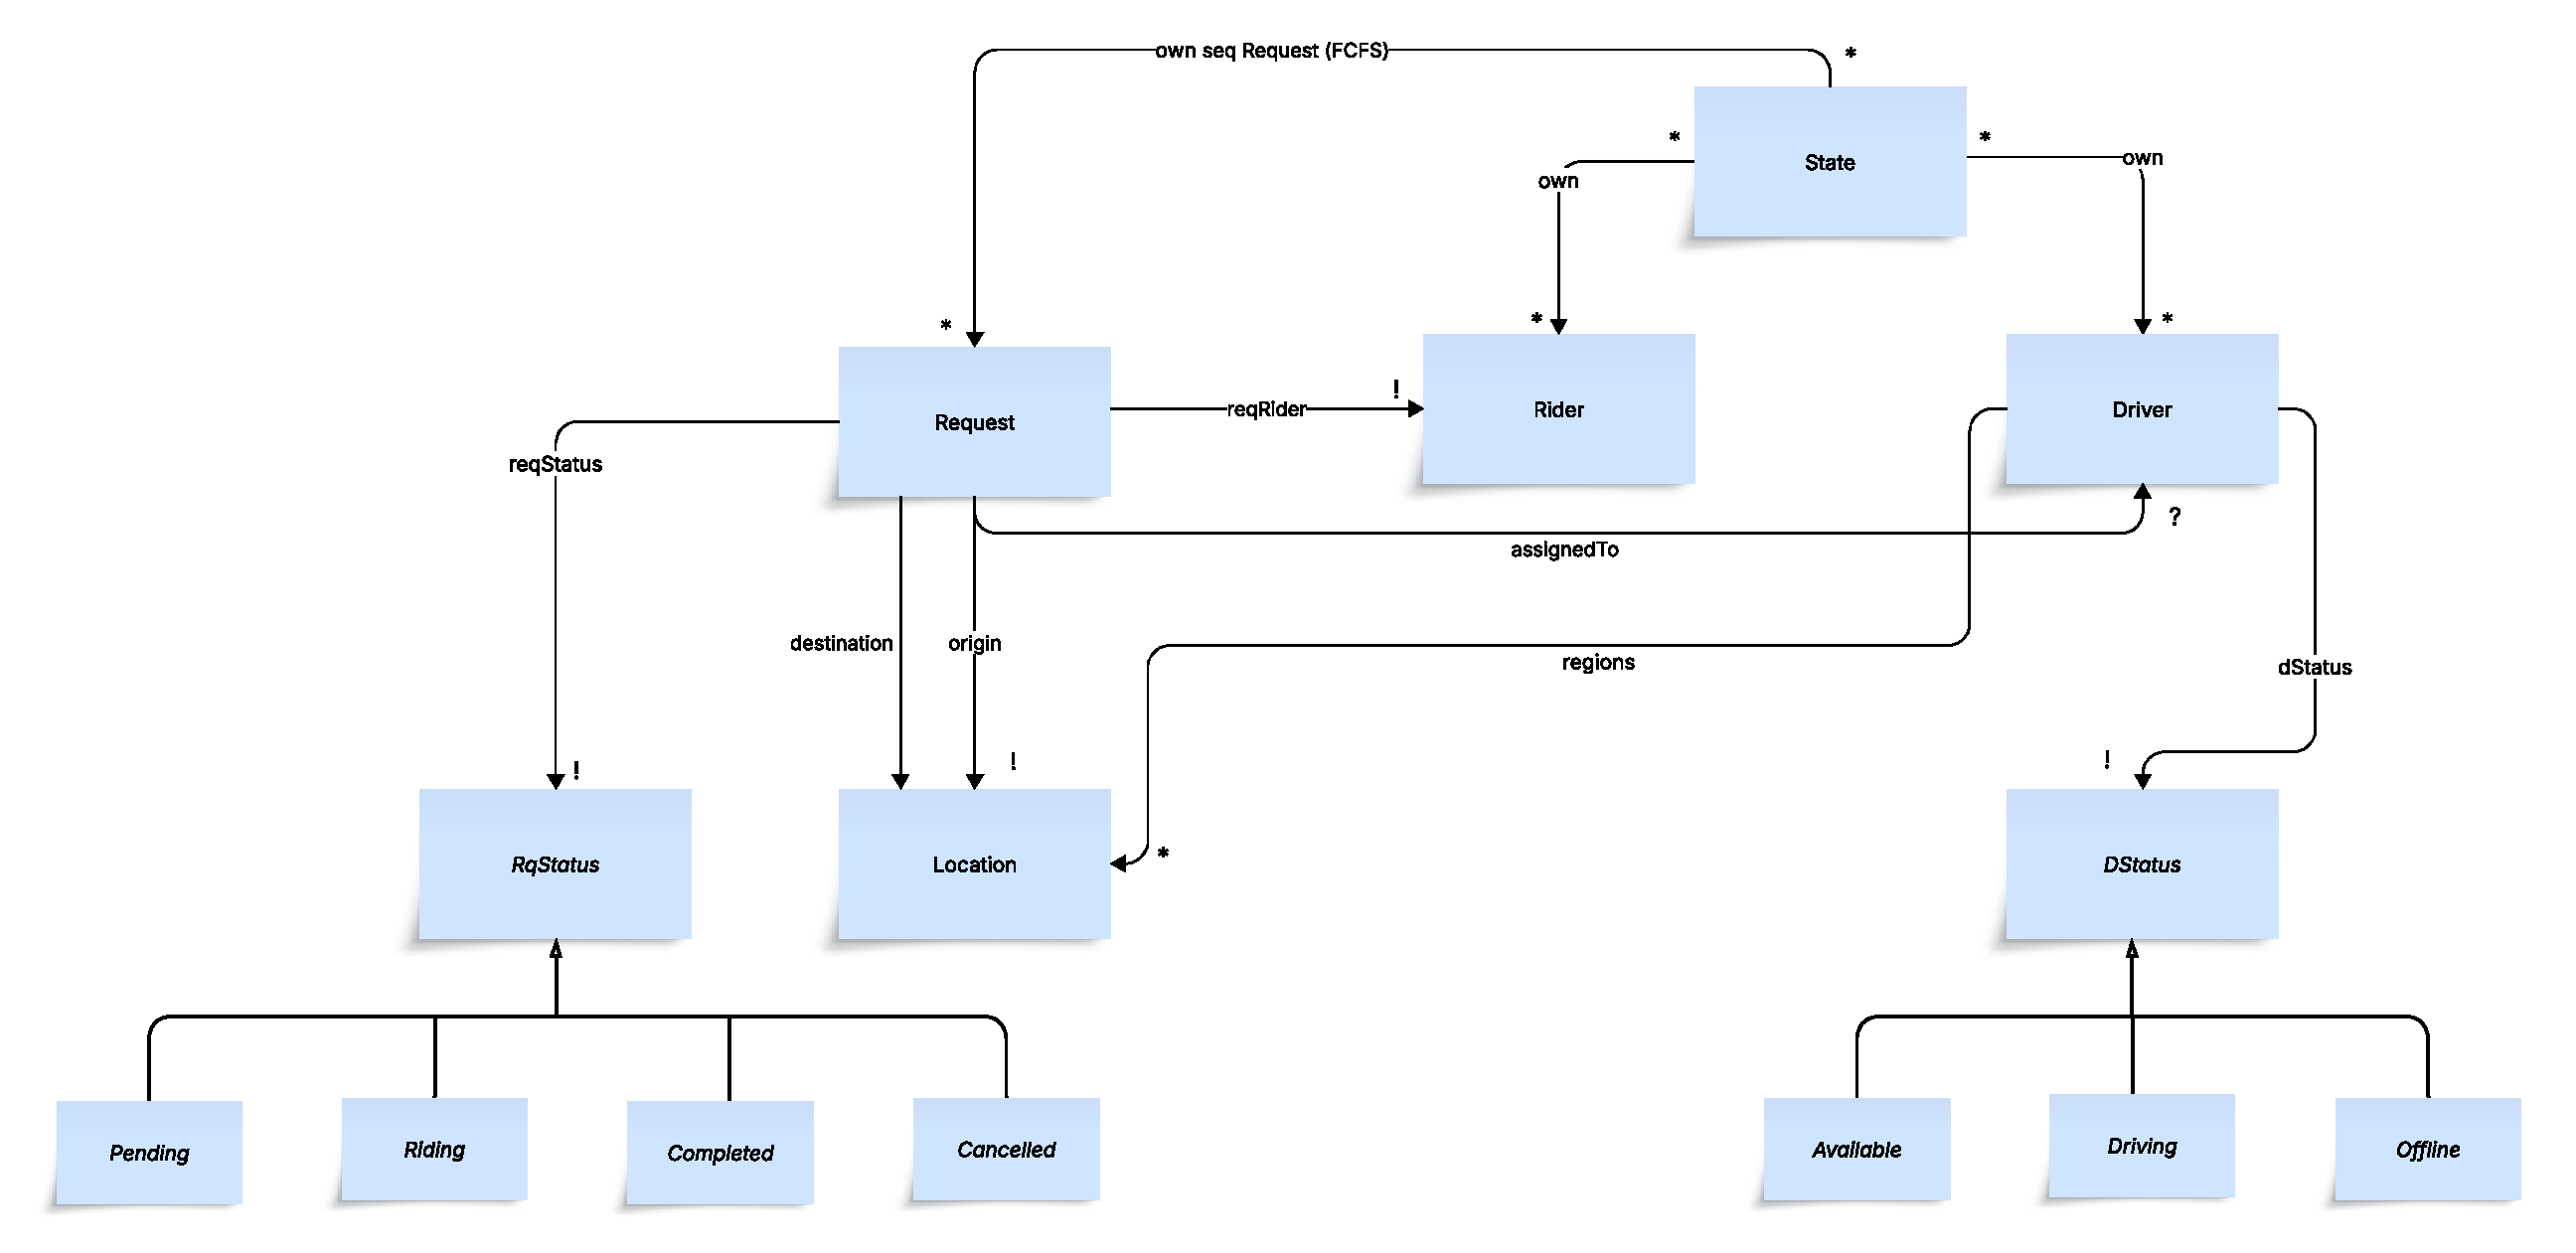
\includegraphics[width=1.00\linewidth]{figs/object-model.pdf}
  \caption{Object model of the \textit{Presto} system.}
\end{figure}

\subsection{Invariants Discovered During Modeling}

During Alloy modeling of \textit{Presto}, we identified several invariants that ensure consistency of the system state:

\begin{itemize}[leftmargin=1.5em]
  \item \textbf{One active request per rider}: Each rider can have at most one request that is either \texttt{Pending} or \texttt{Riding}.
  \item \textbf{Driver exclusivity}: Each driver can serve at most one request at a time. A driver is in the \texttt{Driving} state if and only if they are assigned to exactly one active request.
  \item \textbf{Assignment consistency}: A request in \texttt{Riding} must have exactly one assigned driver. Requests in \texttt{Pending}, \texttt{Completed}, or \texttt{Cancelled} must have no assigned driver.
  \item \textbf{Queue well-formedness}: The set of requests in the \texttt{Pending} state must exactly equal the elements of the \texttt{pendingQ} sequence (with no duplicates).
  \item \textbf{Origin-destination sanity}: For realism, each request must have distinct origin and destination.
\end{itemize}
These invariants capture both explicit rules in the specification and implicit requirements necessary to preserve logical correctness.

\subsection{Model Validation Strategy}

Our validation strategy for the Alloy model involved:
\begin{itemize}[leftmargin=1.5em]
  \item \textbf{Operation preservation checks}: We wrote assertions ensuring that the four core operations (\texttt{request}, \texttt{cancel}, \texttt{match}, and \texttt{complete}) preserve the system invariants across state transitions.
  \item \textbf{Visualization of states}: Using \texttt{run} commands, we generated concrete states, such as an empty system, one pending request, and one riding request. These helped confirm intuitive behavior.
  \item \textbf{Counterexample analysis}: If Alloy produced a counterexample, we refined the model (e.g., corrected scoping errors or missing conditions) until the invariants held.
  \item \textbf{Cross-checking with the spec}: Each invariant and operation was traced back to requirements in the Presto specification to ensure coverage.
\end{itemize}
In addition, we developed a suite of \textbf{positive and negative test predicates} 
to exercise the model further. Positive tests (e.g., \texttt{test\_MultiplePending}, 
\texttt{test\_MultipleConcurrentRides}) confirmed that realistic states were satisfiable, 
while negative tests (e.g., \texttt{test\_RidingRequestInPendingQueue}, 
\texttt{test\_AvailableDriverIsAssigned}, \texttt{test\_DuplicateRequestInQueue}) 
demonstrated that invalid states were impossible under our invariants. 
Running these tests under scopes of 4–7 atoms with exactly one \texttt{State} 
reinforced our confidence that the model was both correct and complete.

\subsection{Scopes for Checking Assertions}

For invariant preservation checks, we used scopes of 6–7 objects with exactly one State and up to 6 sequence elements. 
This bound was sufficient because:
\begin{itemize}[leftmargin=1.5em]
  \item It allowed us to explore diverse combinations of Riders, Drivers, and Requests while keeping the analysis tractable.
  \item Larger scopes (beyond 7) did not uncover new counterexamples, suggesting our invariants are robust.
  \item These bounds match the project’s guidance for balancing coverage with solver performance.
\end{itemize}

\section{Task 2: Concurrency with FSP/LTSA}
\label{sec:task2}

\subsection{Process Structure Diagram}

\label{sec:process-structure}
\begin{figure}[h]
  \centering
  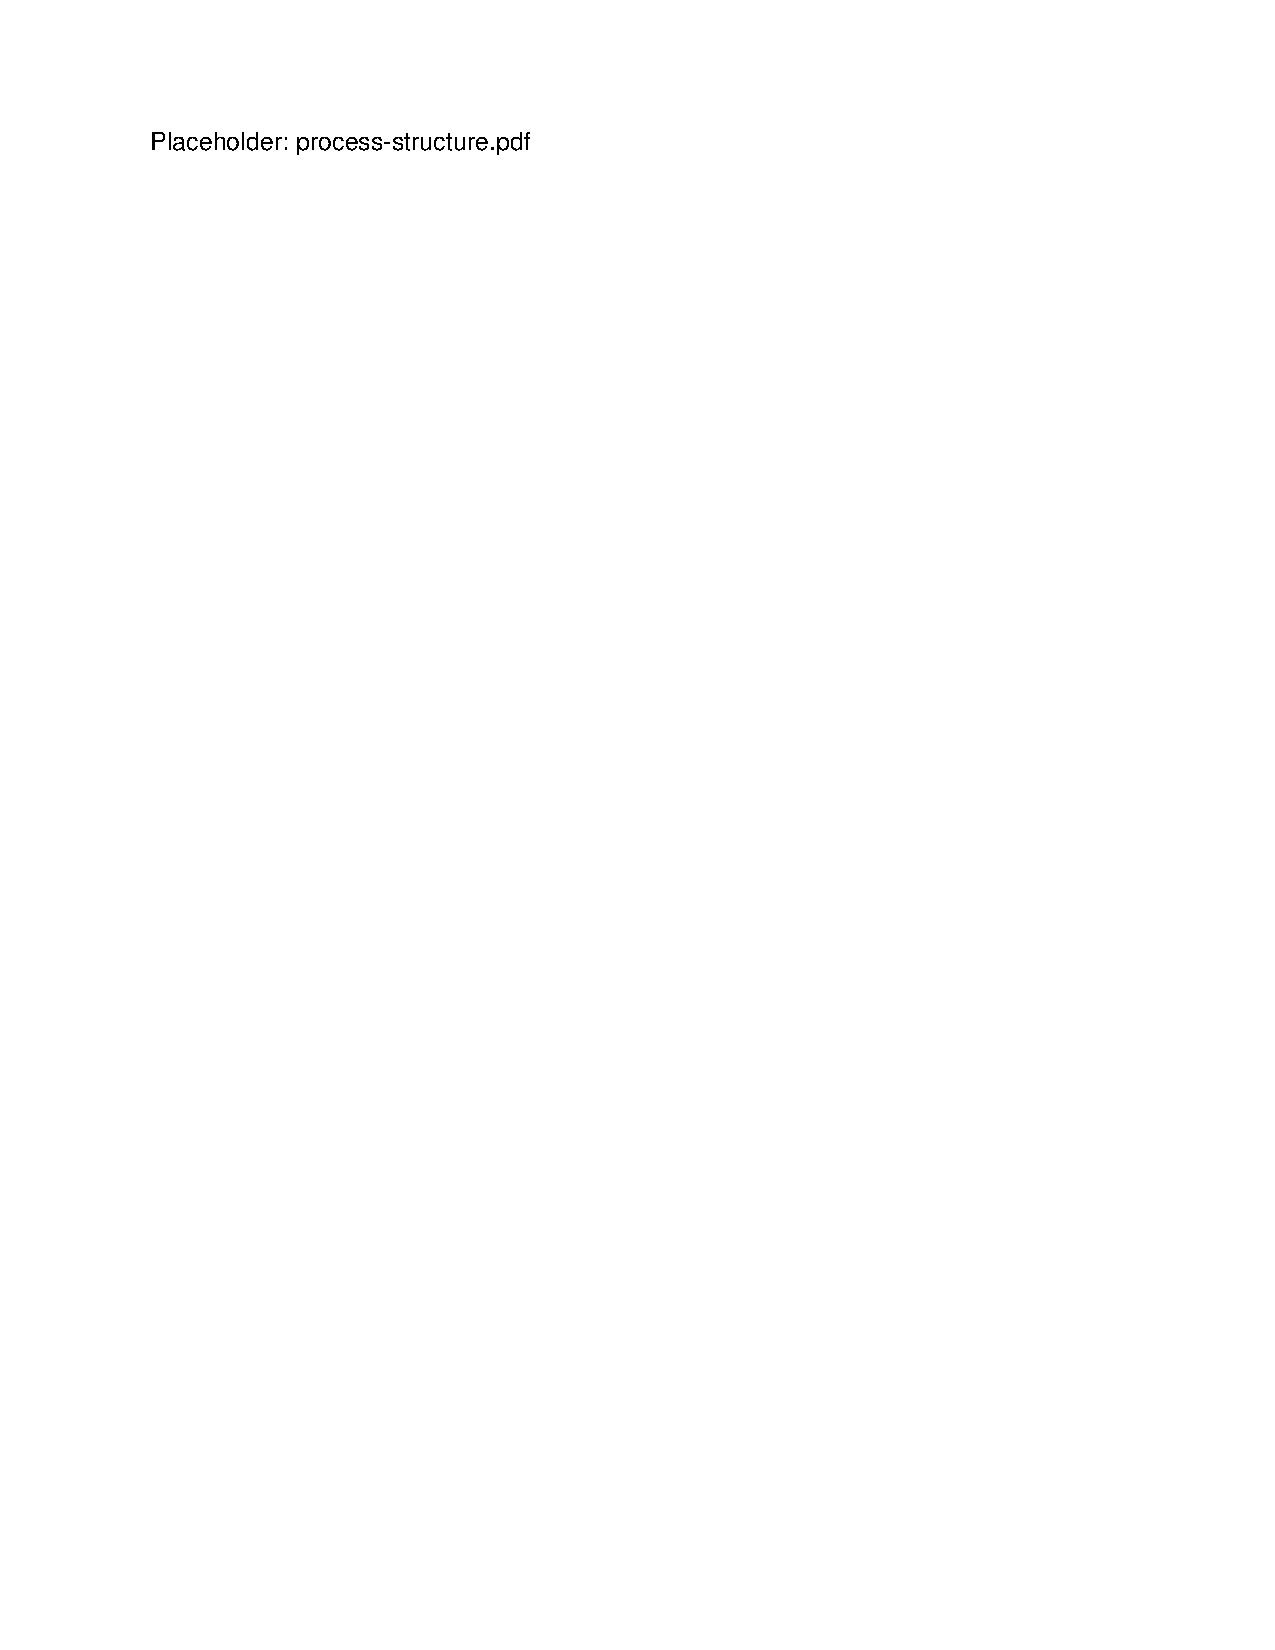
\includegraphics[width=0.50\linewidth]{figs/process-structure.pdf}
  \caption{Process Structure diagram for the FSP model.}
\end{figure}
\begin{itemize}[leftmargin=1.5em]
  \item \textbf{ORDER}: a generator that cycles order identifiers $t \in \{1,\dots,\texttt{NUMRIDER}\}$ and emits \texttt{request[$t$]} in round-robin order.
  \item \textbf{RIDER($i$)} for each $i \in \{1,\dots,\texttt{NUMRIDER}\}$:
    \texttt{request[$i$]} $\rightarrow$ \texttt{match[$i$]} $\rightarrow$ \texttt{complete[$i$]} (or \texttt{cancel[$i$]} before match).
  \item \textbf{SCHEDULER} as a driver pool \texttt{DRIVER($d,t$)}:
    \begin{itemize}[leftmargin=1.2em]
      \item if $d>0$: \texttt{match[$t$]} uses one available driver $\Rightarrow$ \texttt{DRIVER($d{-}1$, next($t$))}
      \item \texttt{cancel[$t$]} skips the slot $\Rightarrow$ \texttt{DRIVER($d$, next($t$))}
      \item if $d<\texttt{NUMDRIVER}$: \texttt{complete[$t$]} returns a driver $\Rightarrow$ \texttt{DRIVER($d{+}1$, $t$)}
    \end{itemize}
\end{itemize}

\noindent The system composition is:
\[
\texttt{ASSIGN\_SYS} = \left(\parallel\, i:\texttt{Order}\, @\, \texttt{RIDER}(i)\right) \parallel \texttt{SCHEDULER} \parallel \texttt{ORDER}.
\]


\subsection{Protocol Design}

\textbf{Events.} We model four observable events with an index $t$ identifying the request/rider:
\texttt{request[$t$]}, \texttt{match[$t$]}, \texttt{cancel[$t$]}, \texttt{complete[$t$]}.

\paragraph{Rider protocol.}
For each rider $i$, the process \texttt{RIDER($i$)} performs \texttt{request[$i$]} then waits
either to be matched (\texttt{match[$i$]}) and subsequently completed (\texttt{complete[$i$]}),
or to cancel before being matched (\texttt{cancel[$i$]}), after which it may request again.

\paragraph{Scheduler / driver pool.}
The scheduler maintains an integer $d$ of available drivers and a rotating pointer $t$.
If $d>0$, the scheduler may synchronize on \texttt{match[$t$]} (consuming one driver and moving to next($t$));
upon \texttt{cancel[$t$]} it skips to next($t$) without consuming a driver; upon \texttt{complete[$t$]},
it returns a driver ($d{+}1$) while keeping $t$ to allow back-to-back completions.

\paragraph{Arrival order (FCFS).}
Arrival order is modeled by \texttt{ORDER} which emits \texttt{request[$t$]} in a round-robin over the index set.
We enforce first-come, first-served with a property automaton \texttt{FIFO\_CHECK} that flags an \texttt{ERROR}
if \texttt{match[2]} occurs before \texttt{match[1]} when 1 arrived first (and symmetrically for two requests).
This is the standard FIFO witness for two requests and is sufficient to catch out-of-order matches.

\subsection{Details Abstracted from Task 1}

Compared to the Alloy state model, the FSP protocol abstracts away:
\begin{itemize}[leftmargin=1.5em]
  \item \textbf{Locations and regions}: We do not carry \texttt{origin}, \texttt{destination}, or driver \texttt{regions}. Region feasibility is left implicit (always matchable when a driver is available).
  \item \textbf{Structural associations}: Fields such as \texttt{reqRider}, \texttt{assignedTo}, and the explicit \texttt{pendingQ} structure are represented behaviorally via indexed events and the scheduler’s pointer $t$.
  \item \textbf{Per-request object identity}: Requests are denoted by indices ($t$) rather than explicit objects; this is sufficient for the concurrency protocol.
\end{itemize}

\subsection{Details Added Beyond Task 1}

The FSP model adds explicit behavioral constraints that Alloy does not natively express:
\begin{itemize}[leftmargin=1.5em]
  \item \textbf{Interleaving semantics}: Competing \texttt{request}, \texttt{match}, \texttt{cancel}, \texttt{complete} events from multiple riders interleave under LTSA’s process-algebra rules.
  \item \textbf{Driver capacity dynamics}: The integer parameter $d$ captures resource consumption at \texttt{match[$t$]} and release at \texttt{complete[$t$]}.
  \item \textbf{Safety property for FCFS}: The \texttt{FIFO\_CHECK} property process rules out any trace where a later request is matched before an earlier one (two-request witness).
  \item \textbf{Progress (liveness)}: We require that completions keep happening via the LTSA progress set \texttt{progress SERVED = \{complete[Order]\}}; optionally, we can strengthen liveness with a per-request watchdog ensuring that after \texttt{request[$i$]} some \texttt{match[$i$]} or \texttt{cancel[$i$]} must occur.
\end{itemize}

\section{Task 3: Reflection}
\label{sec:task3}

\subsection{Alloy: Strengths and Weaknesses}

\textbf{Strengths:}
\begin{itemize}[leftmargin=1.5em]
  \item Naturally suited for modeling structural constraints and invariants.
  \item Immediate visualization of counterexamples, which aids debugging.
  \item Compact and expressive syntax for relational properties.
\end{itemize}
\textbf{Weaknesses:}
\begin{itemize}[leftmargin=1.5em]
  \item Not designed to capture concurrency or event ordering explicitly.
  \item Large scopes can cause performance issues.
  \item Expressing temporal behaviors (e.g., eventuality) requires workarounds.
\end{itemize}

\subsection{FSP/LTSA: Strengths and Weaknesses}

\textbf{Strengths.}
\begin{itemize}[leftmargin=1.5em]
  \item Natural description of concurrent event interleavings and shared synchronizations.
  \item Built-in checks for deadlock and support for progress (liveness) via progress sets.
  \item Property processes (e.g., \texttt{FIFO\_CHECK}) make safety conditions executable.
\end{itemize}

\textbf{Weaknesses.}
\begin{itemize}[leftmargin=1.5em]
  \item Structural constraints (e.g., object associations, multiplicities) are not explicit; they must be encoded behaviorally or left to Alloy.
  \item FIFO beyond the two-request witness requires either a generalized property pattern or a larger monitor, which can grow in complexity.
  \item Liveness per request (``each request eventually served'') often needs additional fairness assumptions or watchdog processes to exclude pathological schedules.
\end{itemize}

\subsection{Other Aspects of Ride Sharing}

While our models capture the core protocol, real-world ride sharing involves additional aspects:
\begin{itemize}[leftmargin=1.5em]
  \item \textbf{Pricing and payment}: Fare calculation, dynamic pricing, and payment handling.
  \item \textbf{Trust and reputation}: Ratings, cancellation penalties, and fraud prevention.
  \item \textbf{Geographic constraints}: Real-world routing, travel times, and multi-region rides.
  \item \textbf{System resilience}: Handling driver disconnections, rider no-shows, or sudden surges.
\end{itemize}

\end{document}